\documentclass{article}

% ---------------------------------------------------------
% 1. SETUP & PACKAGES
% ---------------------------------------------------------
\PassOptionsToPackage{numbers, compress}{natbib}

% [preprint] shows your names. Change to [final] for the final version.
\usepackage[final]{neurips_2024}

% Remove the conference footer from the first page
\makeatletter
\renewcommand{\@noticestring}{}
\makeatother

\usepackage[utf8]{inputenc} % allow utf-8 input
\usepackage[T1]{fontenc}    % use 8-bit T1 fonts
\usepackage[french, provide=*]{babel}  % French language support
\usepackage{hyperref}       % hyperlinks
\usepackage{url}            % simple URL typesetting
\usepackage{booktabs}       % professional-quality tables
\usepackage{amsmath}        % best math environment
\usepackage{amsthm}         % for theorems
\newtheorem{theorem}{Théorème}
\usepackage{amsfonts}       % blackboard math symbols
\usepackage{nicefrac}       % compact symbols for 1/2, etc.
\usepackage[expansion=false]{microtype}      % microtypography
\usepackage{graphicx}       % for images
\usepackage{enumitem}       % for cleaner lists
\usepackage{multirow}
\usepackage{xcolor}         % color text
\usepackage{tikz}
\usetikzlibrary{shapes.geometric, arrows.meta, positioning, calc, decorations.pathreplacing}
\usepackage{pgfplots}
\usepackage{float}
\usepackage{natbib}
\usepackage{amssymb}
\pgfplotsset{compat=1.18}

% Custom Colors
\definecolor{myBlue}{RGB}{70, 130, 180}
\definecolor{myOrange}{RGB}{255, 140, 0}
\definecolor{myGreen}{RGB}{60, 179, 113}


% ---------------------------------------------------------
% 2. TITLE & AUTHORS
% ---------------------------------------------------------
\title{Analyse Comparative Approfondie : IWAE vs VAE, Compromis Biais-Variance et Richesse Latente}

\author{%
  Amine Mike El Maalouf \\
  \texttt{amine.el-maalouf@epita.fr} \\
  \And
  Cedric Damais \\
  \texttt{cedric.damais@epita.fr} \\
  \And
  Yacine Benihaddadene \\
  \texttt{yacine.benihaddadene@epita.fr} \\
  \And
  Leon Ayral \\
  \texttt{leon.ayral@epita.fr} \\
  \And
  Oscar Le Dauphin \\
  \texttt{oscar.le-dauphin@epita.fr} \\
}

\begin{document}

\maketitle

% ---------------------------------------------------------
% 3. ABSTRACT
% ---------------------------------------------------------

\begin{abstract}
Les Autoencodeurs Variationnels (VAE) se sont imposés comme une méthode de référence dans le domaine des modèles génératifs profonds, permettant d'approximer des distributions a posteriori souvent intraitables via la maximisation d'une borne inférieure variationnelle sur l'évidence (ELBO). Néanmoins, la formulation standard de l'objectif du VAE introduit un biais d'approximation qui contraint fréquemment le modèle à converger vers des représentations sous-optimales et excessivement simplifiées, un phénomène connu sous le nom d'effondrement du postérieur. Ce projet de recherche propose une étude exhaustive de l'Importance Weighted Autoencoder (IWAE), une généralisation rigoureuse du VAE qui optimise une borne strictement plus fine sur la log-vraisemblance marginale, dérivée des principes de l'échantillonnage préférentiel (Importance Sampling). Nous analysons en détail l'impact théorique de cet objectif modifié sur la qualité de l'estimation des gradients, la réduction du biais et la flexibilité de la distribution variationnelle implicite. Nos expériences approfondies, menées sur le jeu de données de référence MNIST, démontrent de manière empirique que l'utilisation de multiples échantillons pondérés ($K>1$) améliore significativement la log-vraisemblance par rapport au VAE standard ($K=1$). De surcroît, nos résultats confirment que l'IWAE parvient à exploiter l'espace latent avec une efficacité accrue, augmentant substantiellement le nombre d'unités actives et produisant des représentations sémantiques plus riches et moins compressées. Toutefois, nous investiguons également une limitation critique mise en lumière par la littérature récente : lorsque le nombre d'échantillons $K$ augmente indéfiniment, le rapport signal sur bruit (SNR) des gradients de l'encodeur diminue de manière asymptotique, dégradant potentiellement la capacité d'apprentissage du réseau d'inférence malgré une borne théorique plus serrée.
\end{abstract}

\newpage
% ---------------------------------------------------------
% 4. SECTIONS
% ---------------------------------------------------------
\section{Introduction}

L'avènement de l'apprentissage profond a révolutionné notre capacité à modéliser des distributions de données complexes et de haute dimension. Au cœur de cette révolution, les modèles génératifs profonds occupent une place prépondérante, offrant la possibilité non seulement de classifier ou de discriminer des données existantes, mais également de synthétiser de nouvelles instances réalistes—qu'il s'agisse d'images photoréalistes, de séquences audio cohérentes ou de textes structurés. Parmi les diverses familles de modèles génératifs, qui incluent notamment les Réseaux Antagonistes Génératifs (GANs) et les modèles basés sur les flots (Normalizing Flows), l'Autoencodeur Variationnel (VAE) introduit par \cite{kingma2013auto} se distingue par son élégance théorique. Il propose un cadre unifié combinant la flexibilité d'approximation universelle des réseaux de neurones profonds avec la rigueur probabiliste de l'inférence bayésienne.

Le principe fondamental du VAE repose sur l'apprentissage d'une représentation latente compressée des données, en mappant les observations de l'espace d'entrée vers un espace latent stochastique, puis en reconstruisant ces données. Cette approche permet non seulement la génération, mais aussi l'apprentissage de représentations utiles pour des tâches en aval. Cependant, l'objectif standard du VAE présente des limitations structurelles et inhérentes à son approximation. La borne inférieure sur l'évidence (ELBO), que les VAE cherchent à maximiser, peut s'avérer être une approximation lâche de la véritable log-vraisemblance marginale. Cette divergence survient particulièrement lorsque la famille variationnelle choisie pour le postérieur approché $q_\phi(z|x)$—typiquement une gaussienne diagonale—manque d'expressivité pour capturer la complexité du vrai postérieur $p_\theta(z|x)$. Ce relâchement de la borne conduit fréquemment à des phénomènes pathologiques tels que l'effondrement du postérieur (\textit{posterior collapse}), une situation où le modèle ignore les dimensions latentes informatives et s'appuie entièrement sur la puissance du décodeur autorégressif pour modéliser les données, réduisant ainsi le VAE à un simple modèle de mélange sans structure latente significative.

Pour pallier ces déficiences, l'Importance Weighted Autoencoder (IWAE), introduit par \citet{burda2015importance}, propose une reformulation de l'objectif d'apprentissage. L'IWAE répond à la limitation de la borne ELBO en utilisant l'échantillonnage préférentiel (\textit{Importance Sampling}) pour dériver une borne strictement plus serrée sur la log-vraisemblance. En utilisant plusieurs échantillons pondérés pour estimer le gradient, l'IWAE permet théoriquement au modèle d'accéder à une distribution postérieure implicite beaucoup plus flexible, ne se limitant plus aux contraintes de la forme gaussienne simple.

Dans ce rapport technique détaillé, nous nous proposons d'étudier les fondements mathématiques et théoriques de l'IWAE, en mettant en exergue les mécanismes par lesquels il améliore l'inférence variationnelle. Nous comparons méthodiquement ses performances à celles du VAE standard sur le jeu de données MNIST, en analysant non seulement la vraisemblance finale, mais aussi la dynamique d'apprentissage et l'utilisation des ressources latentes. Enfin, nous explorons à la fois ses avantages indéniables en termes de modélisation et ses inconvénients potentiels, notamment le paradoxe du gradient bruité, avant d'examiner les développements récents de la recherche qui ont construit sur le cadre de l'IWAE pour repousser les limites de l'inférence variationnelle.

% ---------------------------------------------------------
\section{Contexte Théorique et Fondations Mathématiques}

Pour comprendre les nuances qui distinguent l'IWAE du VAE standard, il est impératif de revenir aux premiers principes des modèles à variables latentes et de l'inférence variationnelle.

\subsection{Le Paradigme des Modèles à Variables Latentes}

L'apprentissage profond génératif, dans son approche probabiliste, repose sur l'hypothèse fondamentale de la variété (\textit{Manifold Hypothesis}). Cette hypothèse stipule que les données de haute dimension que nous observons dans le monde réel, telles que des images ou des signaux sonores, ne remplissent pas uniformément l'espace d'entrée (par exemple, l'espace des pixels $\mathbb{R}^{784}$ pour MNIST). Au contraire, elles se concentrent sur des sous-variétés non linéaires de dimension beaucoup plus faible, imbriquées dans cet espace de haute dimension.

Soit $\mathcal{D} = \{x^{(i)}\}_{i=1}^N$ un ensemble de données composé d'observations indépendantes et identiquement distribuées (i.i.d.) d'une variable aléatoire continue ou discrète $x \in \mathcal{X}$. Nous postulons que ces données sont générées par un processus aléatoire causal, non observé directement, impliquant une variable latente continue $z \in \mathcal{Z}$. La dimension de cet espace latent est typiquement très inférieure à celle des données observables ($\text{dim}(z) \ll \text{dim}(x)$), forçant le modèle à capturer les facteurs de variation les plus saillants (forme, couleur, orientation, etc.). Le processus génératif conjoint est défini par la factorisation suivante :
\begin{equation}
    p_\theta(x, z) = p_\theta(x|z)p(z)
\end{equation}

Dans cette formulation :
\begin{itemize}
    \item $p(z)$ représente la distribution a priori (\textit{prior}) sur les variables latentes. Pour des raisons de simplicité analytique et de régularité, elle est souvent fixée comme une loi normale standard multivariée isotrope, $\mathcal{N}(0, I)$.
    \item $p_\theta(x|z)$ représente la distribution de vraisemblance conditionnelle (\textit{likelihood}), modélisée par une fonction paramétrique complexe—un réseau de neurones profond—dont les paramètres sont notés $\theta$. Ce composant est souvent appelé le \textit{décodeur} ou le \textit{modèle génératif}, car il apprend la transformation non linéaire permettant de projeter un point de l'espace latent abstrait vers l'espace des données observables.
\end{itemize}

\subsection{Le Problème de l'Intractabilité de l'Évidence}

L'objectif central de l'apprentissage dans ce cadre est de maximiser la vraisemblance des données observées. Cela nécessite de calculer la vraisemblance marginale (ou évidence), notée $p_\theta(x)$, qui s'obtient en marginalisant (intégrant) la variable latente $z$ hors de la distribution conjointe :
\begin{equation}
    p_\theta(x) = \int_{\mathcal{Z}} p_\theta(x, z) \, dz = \int_{\mathcal{Z}} p_\theta(x|z)p(z) \, dz
\end{equation}

Cette intégrale constitue le nœud du problème. Pour des modèles profonds où la dépendance $x|z$ est paramétrée par un réseau de neurones non linéaire à plusieurs couches, cette intégrale ne possède pas de solution analytique fermée. De plus, l'espace $\mathcal{Z}$ étant continu et potentiellement de haute dimension, les méthodes d'intégration numérique classiques (quadrature) sont inopérantes en raison du fléau de la dimensionnalité.

Cette intractabilité de $p_\theta(x)$ a une conséquence directe : elle rend impossible le calcul exact de la distribution a posteriori $p_\theta(z|x)$ via la règle de Bayes :
\begin{equation}
    p_\theta(z|x) = \frac{p_\theta(x|z)p(z)}{p_\theta(x)}
\end{equation}
Puisque le dénominateur est inconnu, nous ne pouvons pas évaluer directement quelle configuration latente $z$ a probablement généré une donnée $x$ spécifique.

\subsection{L'Inférence Variationnelle Amortie (Amortized VI)}

Pour contourner l'intractabilité du vrai postérieur, l'Inférence Variationnelle (VI) transforme le problème d'intégration en un problème d'optimisation. L'idée est d'approcher le vrai postérieur $p_\theta(z|x)$ par une famille de distributions paramétriques plus simples, notée $q_\phi(z|x)$, appelée \textit{distribution variationnelle} ou \textit{réseau d'inférence} (encodeur), dont les paramètres sont notés $\phi$.

Contrairement aux méthodes variationnelles classiques qui optimiseraient un paramètre variationnel distinct pour chaque point de donnée (ce qui serait prohibitif pour de grands ensembles de données), les VAE utilisent l'\textit{inférence amortie}. Un seul réseau de neurones (l'encodeur) apprend à prédire les paramètres de la distribution variationnelle $\phi = f(x)$ pour n'importe quelle entrée $x$.

L'objectif est de trouver les paramètres $\phi$ qui minimisent la divergence entre l'approximation et la vraie distribution. La métrique standard utilisée en théorie de l'information pour mesurer la dissimilarité entre deux distributions de probabilité est la divergence de Kullback-Leibler (KL) :
\begin{equation}
    \mathbb{KL}(q_\phi(z|x) || p_\theta(z|x)) = \int q_\phi(z|x) \log \frac{q_\phi(z|x)}{p_\theta(z|x)} \, dz = \mathbb{E}_{z \sim q_\phi} \left[ \log q_\phi(z|x) - \log p_\theta(z|x) \right]
\end{equation}

Cependant, minimiser directement cette divergence KL est impossible car elle dépend du terme inconnu $p_\theta(z|x)$ (et donc de $p_\theta(x)$).

\subsection{Dérivation Formelle de la Borne Inférieure (ELBO)}

Nous pouvons reformuler le problème en analysant la log-vraisemblance marginale. En utilisant les propriétés du logarithme et de l'espérance, nous avons l'identité suivante pour tout $z$ tel que $q_\phi(z|x) > 0$ :
\begin{equation}
    \log p_\theta(x) = \mathbb{E}_{z \sim q_\phi} [\log p_\theta(x)]
\end{equation}
En appliquant la règle de Bayes à l'intérieur de l'espérance ($p_\theta(x) = p_\theta(x,z) / p_\theta(z|x)$) et en multipliant par l'identité $1 = \frac{q_\phi(z|x)}{q_\phi(z|x)}$, nous obtenons :

\begin{align}
    \log p_\theta(x) &= \mathbb{E}_{z \sim q_\phi} \left[ \log \frac{p_\theta(x, z)}{p_\theta(z|x)} \right] \\
    &= \mathbb{E}_{q_\phi} \left[ \log \left( \frac{p_\theta(x, z)}{q_\phi(z|x)} \cdot \frac{q_\phi(z|x)}{p_\theta(z|x)} \right) \right] \\
    &= \underbrace{\mathbb{E}_{q_\phi} \left[ \log \frac{p_\theta(x, z)}{q_\phi(z|x)} \right]}_{\mathcal{L}_{\text{ELBO}}(\theta, \phi; x)} + \underbrace{\mathbb{E}_{q_\phi} \left[ \log \frac{q_\phi(z|x)}{p_\theta(z|x)} \right]}_{\mathbb{KL}(q_\phi(z|x) || p_\theta(z|x))}
\end{align}

Cette décomposition est fondamentale. Elle relie la quantité que nous voulons maximiser ($\log p_\theta(x)$), une quantité que nous pouvons calculer ($\mathcal{L}_{\text{ELBO}}$), et l'erreur d'approximation ($\mathbb{KL}$).
Puisque la divergence KL est, par définition, toujours positive ou nulle (inégalité de Gibbs), le terme $\mathcal{L}_{\text{ELBO}}$ constitue mathématiquement une borne inférieure stricte sur la log-vraisemblance des données :
\begin{equation}
    \log p_\theta(x) \ge \mathcal{L}_{\text{ELBO}}(\theta, \phi; x)
\end{equation}

L'égalité $\log p_\theta(x) = \mathcal{L}_{\text{ELBO}}$ n'est atteinte que si et seulement si $q_\phi(z|x) = p_\theta(z|x)$ presque partout, c'est-à-dire si notre approximation variationnelle est parfaite.

\subsection{Le VAE Standard et l'Astuce de Reparamétrisation}

Le VAE maximise cette borne ELBO par descente de gradient stochastique. L'ELBO peut être réécrite sous une forme plus intuitive en séparant les termes d'espérance :
\begin{equation}
    \mathcal{L}_{\text{ELBO}} = \mathbb{E}_{q_\phi(z|x)} [\log p_\theta(x|z)] - \mathbb{KL}(q_\phi(z|x) || p(z))
\end{equation}

Cette formulation met en lumière le double objectif antagoniste du VAE :
1.  \textbf{Terme de Reconstruction :} $\mathbb{E}_{q_\phi(z|x)} [\log p_\theta(x|z)]$ encourage le décodeur à reconstruire fidèlement les données, minimisant ainsi l'erreur de reconstruction (par exemple, l'erreur quadratique moyenne pour un décodeur gaussien ou l'entropie croisée pour Bernoulli).
2.  \textbf{Terme de Régularisation :} $-\mathbb{KL}(q_\phi(z|x) || p(z))$ agit comme un régularisateur, forçant la distribution latente apprise $q_\phi$ à rester proche du prior $p(z)$ (normalement $\mathcal{N}(0, I)$). Cela assure la continuité de l'espace latent et permet la génération par échantillonnage du prior.

Pour optimiser cette fonction objectif via la rétropropagation, le gradient doit pouvoir traverser l'opération d'échantillonnage stochastique $z \sim q_\phi(z|x)$. C'est ici qu'intervient l'\textbf{astuce de reparamétrisation} (\textit{Reparameterization Trick}). Au lieu d'échantillonner directement $z$, nous exprimons $z$ comme une fonction déterministe et différentiable des paramètres $\phi$ (ici $\mu$ et $\sigma$) et d'une variable aléatoire auxiliaire indépendante $\epsilon$ :
\begin{equation}
    z = \mu_\phi(x) + \sigma_\phi(x) \odot \epsilon, \quad \text{avec } \epsilon \sim \mathcal{N}(0, I)
\end{equation}
Cette transformation permet de sortir l'aléa du graphe de computation des gradients par rapport à $\phi$, rendant l'apprentissage de bout en bout possible.

\subsection{Limitations du VAE : Le Fossé d'Approximation}

Bien que puissant, le VAE souffre de la rigidité de sa distribution variationnelle. L'écart entre la vraie log-vraisemblance et l'ELBO est précisément la divergence KL entre les postérieurs approché et vrai :
\begin{equation}
    \log p_\theta(x) - \mathcal{L}_{\text{VAE}} = \text{KL}(q_\phi(z|x) \| p_\theta(z|x))
\end{equation}

Lorsque le vrai postérieur $p_\theta(z|x)$ est complexe (multimodal, asymétrique), une simple gaussienne diagonale $q_\phi(z|x)$ échoue à l'approcher correctement. Ce fossé d'approximation (Gap) reste grand, signifiant que même si nous maximisons parfaitement l'ELBO, nous ne maximisons pas nécessairement $\log p_\theta(x)$. Ce phénomène est un facteur clé de l'\textbf{effondrement du postérieur}, où le terme KL domine l'optimisation et pousse $q_\phi$ vers le prior $p(z)$, rendant $z$ indépendant de $x$ et forçant le décodeur à agir comme un modèle inconditionnel.

% ---------------------------------------------------------
\section{La Solution IWAE : Une Généralisation par l'Échantillonnage Préférentiel}

L'Importance Weighted Autoencoder (IWAE), proposé par \citet{burda2015importance}, ne se contente pas d'être une simple extension incrémentale du VAE ; il représente un pont conceptuel fondamental entre l'Inférence Variationnelle (VI) et les méthodes de Monte Carlo (Importance Sampling). Il répond structurellement au relâchement de la borne ELBO en exploitant la capacité de l'échantillonnage préférentiel à corriger les inadéquations entre la distribution de proposition (l'encodeur) et la distribution cible.

\subsection{L'Objectif IWAE : Une Perspective Monte Carlo}

L'innovation centrale de l'IWAE réside dans la définition de son objectif. Au lieu d'utiliser un seul échantillon pour estimer l'ELBO (comme c'est souvent le cas dans le VAE stochastique standard), l'IWAE construit un estimateur de la vraisemblance marginale $p_\theta(x)$ basé sur la moyenne de $K$ rapports de densité.
L'objectif à maximiser est défini par :

\begin{equation}
    \mathcal{L}_K(x) = \mathbb{E}_{z_1, \ldots, z_K \sim q_\phi(z|x)} \left[ \log \left( \frac{1}{K} \sum_{i=1}^{K} w_i \right) \right]
\end{equation}

où les \textit{poids d'importance non normalisés} sont définis par le rapport entre la distribution conjointe et la distribution variationnelle pour chaque échantillon $i$ :
\begin{equation}
    w_i = \frac{p_\theta(x, z_i)}{q_\phi(z_i|x)} = \frac{p_\theta(x|z_i)p(z_i)}{q_\phi(z_i|x)}
\end{equation}

Intuitivement, la quantité $\frac{1}{K} \sum w_i$ est un estimateur de Monte Carlo non biaisé de l'évidence $p_\theta(x)$. En effet, $\mathbb{E}[w_i] = \int \frac{p(x,z)}{q(z|x)}q(z|x) dz = \int p(x,z) dz = p(x)$.
Cependant, comme nous optimisons le logarithme de cette quantité (pour des raisons de stabilité numérique et d'adaptation aux fonctions de perte des réseaux de neurones), l'estimateur devient biaisé. Selon l'inégalité de Jensen concave ($\mathbb{E}[\log X] \le \log \mathbb{E}[X]$), $\mathcal{L}_K$ est une borne inférieure de $\log p_\theta(x)$. L'IWAE cherche à réduire ce biais en augmentant le nombre d'échantillons $K$.

\subsubsection{Cohérence Théorique : Le Cas Limite $K=1$}

Un impératif de cohérence pour toute généralisation est de retrouver le modèle original dans ses cas limites. Il est donc instructif de démontrer formellement que l'objectif IWAE se réduit exactement à la borne ELBO standard du VAE lorsque le budget d'échantillonnage est restreint à une unique particule ($K=1$).

Partons de la définition de la borne IWAE donnée précédemment :
\begin{equation}
    \mathcal{L}_K(x) = \mathbb{E}_{z_{1:K} \sim q_\phi(z|x)} \left[ \log \left( \frac{1}{K} \sum_{i=1}^{K} \frac{p_\theta(x, z_i)}{q_\phi(z_i|x)} \right) \right]
\end{equation}

En posant $K=1$, la somme se réduit à un seul terme et le facteur de normalisation $1/K$ devient $1$. L'espérance ne porte plus que sur une seule variable aléatoire $z_1$. L'expression se simplifie alors immédiatement :

\begin{align}
    \mathcal{L}_1(x) &= \mathbb{E}_{z_1 \sim q_\phi(z|x)} \left[ \log \left( \frac{1}{1} \sum_{i=1}^{1} \frac{p_\theta(x, z_i)}{q_\phi(z_i|x)} \right) \right] \\
    &= \mathbb{E}_{z \sim q_\phi(z|x)} \left[ \log \frac{p_\theta(x, z)}{q_\phi(z|x)} \right] \\
    &= \mathbb{E}_{z \sim q_\phi(z|x)} \left[ \log p_\theta(x, z) - \log q_\phi(z|x) \right]
\end{align}

Nous reconnaissons ici très exactement la définition canonique de la borne inférieure de l'évidence (ELBO) utilisée dans le VAE standard :
\begin{equation}
    \mathcal{L}_1(x) \equiv \mathcal{L}_{\text{VAE}}(x)
\end{equation}

Cette équivalence démontre que l'IWAE est une généralisation stricte du VAE. Par conséquent, toute propriété démontrée pour l'IWAE avec $K$ arbitraire s'applique au VAE comme cas particulier dégénéré. Cela implique également que l'amélioration de la borne observée pour $K > 1$ est purement attribuable à la réduction de la variance de l'estimateur et à l'assouplissement des contraintes variationnelles, et non à un changement de paradigme fondamental.

\subsection{Nouveauté 1 : Des Bornes Strictement Plus Serrées}

La contribution théorique majeure de \cite{burda2015importance} est la preuve formelle que l'augmentation du nombre d'échantillons $K$ resserre strictement la borne inférieure. Ce résultat transforme le nombre d'échantillons, auparavant un simple hyperparamètre de variance, en un paramètre de capacité du modèle.

\begin{theorem}[Monotonie de la Borne]
Pour tout $K \ge 1$, la borne IWAE $\mathcal{L}_K$ est minorée par $\mathcal{L}_{K-1}$ et majorée par la log-vraisemblance réelle, convergeant vers cette dernière lorsque $K \to \infty$ :
\begin{equation}
    \mathcal{L}_1 \leq \mathcal{L}_2 \leq \cdots \leq \mathcal{L}_K \leq \log p_\theta(x)
\end{equation}
\end{theorem}

Cela implique que l'IWAE permet d'échanger de la puissance de calcul (plus de $K$, donc plus de passes avant dans le décodeur) contre une meilleure approximation de la log-vraisemblance, sans nécessiter de changement dans l'architecture paramétrique du modèle. Le VAE standard correspond simplement au cas particulier où $K=1$.

\subsubsection{Démonstration Formelle : Croissance Monotone}

Nous présentons ici une preuve formalisée utilisant la technique du sous-ensemble imaginaire, qui offre une intuition claire sur le mécanisme de réduction de biais.

Soit un ensemble d'indices $S_K = \{1, \dots, K\}$. Considérons un sous-ensemble $I \subset S_K$ de taille $m < K$, choisi uniformément parmi tous les sous-ensembles possibles.
Nous utilisons l'observation suivante sur les moyennes empiriques :
\begin{equation}
    \frac{1}{K} \sum_{i=1}^K w_i = \mathbb{E}_{I} \left[ \frac{1}{m} \sum_{j \in I} w_j \right]
\end{equation}
Cette égalité stipule simplement que la moyenne globale est l'espérance de la moyenne d'un sous-échantillon aléatoire.

En substituant cette égalité dans la définition de $\mathcal{L}_K$ et en appliquant l'inégalité de Jensen (la fonction logarithme étant strictement concave) :

\begin{align}
\mathcal{L}_K &= \mathbb{E}_{z_{1 \dots K}} \left[ \log \left( \frac{1}{K} \sum_{i=1}^K w_i \right) \right] \\
&= \mathbb{E}_{z_{1 \dots K}} \left[ \log \left( \mathbb{E}_{I \subset \{1 \dots K\}, |I|=m} \left[ \frac{1}{m} \sum_{j \in I} w_j \right] \right) \right] \\
&\geq \mathbb{E}_{z_{1 \dots K}} \left[ \mathbb{E}_{I} \left[ \log \left( \frac{1}{m} \sum_{j \in I} w_j \right) \right] \right] \quad \text{(par Jensen)} \\
&= \mathbb{E}_{I} \left[ \mathbb{E}_{z_{1 \dots K}} \left[ \log \left( \frac{1}{m} \sum_{j \in I} w_j \right) \right] \right]
\end{align}

Puisque les échantillons $z_i$ sont i.i.d., l'espérance interne ne dépend que des $m$ échantillons indexés par $I$. Par symétrie, peu importe quel ensemble $I$ est choisi, l'espérance est identique et correspond exactement à la définition de $\mathcal{L}_m$. Ainsi, nous avons prouvé que $\mathcal{L}_K \ge \mathcal{L}_m$ pour tout $K > m$.

\subsection{Nouveauté 2 : Le Postérieur Implicite et la Dynamique des Gradients}

Contrairement au VAE qui force le postérior explicite $q_\phi(z|x)$ à correspondre au vrai postérior $p_\theta(z|x)$ (souvent unimodal et complexe), l'IWAE introduit une distribution beaucoup plus flexible appelée \textit{postérior corrigé par l'importance} (Importance Weighted Posterior).

\subsubsection{Les Poids Normalisés comme Mécanisme de Filtrage}
Définissons les poids d'importance normalisés $\tilde{w}_i$, qui jouent un rôle crucial dans l'interprétation du modèle :
\begin{equation}
    \tilde{w}_i = \frac{w_i}{\sum_{j=1}^K w_j}, \quad \text{avec } \sum_{i=1}^K \tilde{w}_i = 1
\end{equation}

Ces poids quantifient la qualité relative de chaque échantillon $z_i$.
Si $z_i$ est un "mauvais" échantillon c'est-à-dire une valeur latente qui conduit à une mauvaise reconstruction $p(x|z)$ ou qui est très improbable sous le prior alors le poids non normalisé $w_i$ sera faible, et par conséquent $\tilde{w}_i \to 0$. Inversement, si $z_i$ est proche de la vraie configuration latente expliquant $x$, $\tilde{w}_i$ dominera la somme.

L'approximation implicite du postérior par l'IWAE, notée $q_{EW}(z|x)$, est une mixture non paramétrique qui converge vers le vrai postérior lorsque $K \to \infty$ :
\begin{equation}
    q_{EW}(z|x) \approx \sum_{i=1}^K \tilde{w}_i \delta(z - z_i) \xrightarrow{K \to \infty} p_\theta(z|x)
\end{equation}

\subsubsection{Analyse Fine du Gradient}
L'impact de ce mécanisme de re-pondération est directement visible dans le calcul du gradient pour l'encodeur $\phi$. En utilisant l'astuce de reparamétrisation ($z_i = \mu + \sigma \odot \epsilon_i$), le gradient de la fonction objectif par rapport à $\phi$ devient :

\begin{equation}
    \nabla_\phi \mathcal{L}_K = \mathbb{E}_{\epsilon_{1:K}} \left[ \sum_{i=1}^{K} \tilde{w}_i \nabla_\phi \log w(x, z_i(\phi)) \right]
\end{equation}

Cette équation révèle une différence comportementale cruciale avec le VAE :
\begin{itemize}
    \item Dans un \textbf{VAE} ($K=1$), nous avons trivialement $\tilde{w}_1 = 1$. Le gradient est calculé aveuglément sur l'échantillon unique, qu'il soit bon ou mauvais. Si l'échantillon est mauvais, le modèle doit ajuster ses paramètres drastiquement pour s'adapter à cette aberration.
    \item Dans un \textbf{IWAE} ($K>1$), le terme $\tilde{w}_i$ agit comme une pondération d'attention automatique. Les gradients provenant de "mauvais" échantillons (faible vraisemblance) sont multipliés par un poids proche de 0 et sont donc effectivement ignorés lors de la mise à jour. Le modèle apprend principalement des "meilleurs" échantillons parmi les $K$ proposés.
\end{itemize}

\subsection{Interprétation : Le Filet de Sécurité (Safety Net)}

L'intuition clé derrière la robustesse de l'IWAE peut être conceptualisée comme un effet de "filet de sécurité".

Dans un VAE standard, si l'encodeur échantillonne une valeur $z$ très improbable (dans les queues de distribution), le terme $\log p(x|z)$ devient extrêmement négatif (par exemple, $-\infty$ en précision machine), causant une variance massive dans les gradients et déstabilisant l'optimisation.

Avec l'IWAE, la structure logarithme-somme-exponentielle offre une protection. Tant qu'au moins \textit{un} des $K$ échantillons tombe dans une région de haute probabilité, la moyenne $\sum w_i$ reste stable. Mathématiquement, la somme à l'intérieur du logarithme empêche l'effondrement vers $-\infty$ :
\begin{equation}
    \log(w_{\text{mauvais}} + w_{\text{bon}}) \approx \log(w_{\text{bon}}) \gg \log(w_{\text{mauvais}})
\end{equation}

Cela permet à l'encodeur d'explorer l'espace latent avec moins de risque, favorisant une couverture plus large des modes de la distribution (\textit{Mode Covering}) plutôt que de se concentrer frileusement sur un seul mode (\textit{Mode Seeking}) comme le fait souvent la divergence KL standard inversée.

\subsection{Le Paradoxe du SNR et la Critique de Rainforth}

Malgré ses avantages, l'IWAE cache une pathologie subtile qui n'apparaît que lors de l'analyse asymptotique. Lorsque $K \to \infty$, quelque chose de contre-intuitif se produit pour l'apprentissage du réseau d'inférence. Considérons le comportement limite des poids normalisés $\tilde{w}_i$ :

\begin{itemize}
    \item À mesure que $K$ augmente, la distribution des poids d'importance devient de plus en plus piquée (concentrée) : typiquement un seul échantillon aura $\tilde{w}_i \approx 1$ tandis que tous les autres auront $\tilde{w}_j \approx 0$. C'est le phénomène connu de dégénérescence des poids en Importance Sampling.
    \item La mise à jour du gradient est alors dominée par ce seul échantillon ``gagnant''.
    \item Le problème est que cet échantillon gagnant est de plus en plus déterminé par le produit de l'a priori $p(z)$ et de la vraisemblance $p_\theta(x|z)$, et non par la qualité de l'encodeur $q_\phi(z|x)$.
\end{itemize}

Mathématiquement, lorsque $K \to \infty$, l'objectif IWAE converge vers la vraie log-vraisemblance :
\begin{equation}
    \mathcal{L}_\infty = \log p_\theta(x) = \log \mathbb{E}_{z \sim q_\phi}[w(x, z)]
\end{equation}

À cette limite, l'objectif ne dépend plus des paramètres $\phi$ de l'encodeur, sauf pour définir le support de l'échantillonnage. Tant que $q_\phi(z|x) > 0$ partout où $p_\theta(x,z) > 0$, la borne est exacte et sa dérivée par rapport à $\phi$ est nulle. Cela signifie que le signal de gradient utile pour entraîner $\phi$ disparaît progressivement.

\subsubsection{Analyse Quantitative du Rapport Signal sur Bruit}

Le Rapport Signal sur Bruit (SNR) de l'estimateur de gradient pour l'encodeur peut être défini comme le ratio entre la magnitude de l'espérance du gradient et son écart-type :
\begin{equation}
    \text{SNR}(\nabla_\phi \mathcal{L}_K) = \frac{|\mathbb{E}[\nabla_\phi \mathcal{L}_K]|}{\text{Std}[\nabla_\phi \mathcal{L}_K]}
\end{equation}

Les travaux fondateurs de \citet{rainforth2018tighter} ont montré un résultat théorique surprenant : tandis que le SNR pour le décodeur $\theta$ augmente avec $K$ (le modèle génératif apprend mieux), le SNR pour l'encodeur $\phi$ diminue avec $K$. Plus précisément :
\begin{equation}
    \text{SNR}(\nabla_\phi \mathcal{L}_K) = \mathcal{O}(K^{-1/2})
\end{equation}

Cela signifie que bien que nous obtenions une meilleure estimation de la valeur de la log-vraisemblance, l'encodeur reçoit des signaux de gradient de plus en plus bruités et faibles par rapport à la variance inhérente à l'échantillonnage.

\subsection{Implications Pratiques du Paradoxe}

Cette dégradation du SNR a des conséquences importantes pour la conception des modèles :
\begin{itemize}
    \item \textbf{Le décodeur apprend bien :} Le modèle génératif $p_\theta(x|z)$ continue de s'améliorer avec un $K$ plus grand, produisant des échantillons plus réalistes.
    \item \textbf{L'encodeur peut stagner :} Le réseau d'inférence $q_\phi(z|x)$ reçoit des signaux de gradient diminuants et peut échouer à s'améliorer, ou converger très lentement.
\end{itemize}

Cette analyse suggère que simplement augmenter $K$ n'est pas une panacée. L'objectif IWAE crée une asymétrie fondamentale où le décodeur bénéficie de plus d'échantillons tandis que l'encodeur en souffre potentiellement.

% ---------------------------------------------------------
\section{Méthodologie Expérimentale et Protocole}

Cette section détaille avec précision le protocole expérimental mis en œuvre pour comparer empiriquement les performances du VAE standard et de l'IWAE. L'objectif est de quantifier le compromis complexe entre la qualité de l'estimation de la vraisemblance, l'utilisation effective de l'espace latent et le coût computationnel associé.

\subsection{Jeu de Données et Prétraitement Avancé}

Nous utilisons le jeu de données standard **MNIST** (Modified National Institute of Standards and Technology), constitué de 70 000 images en niveaux de gris de chiffres manuscrits, de taille 28x28 pixels. Bien que simple, ce dataset reste un benchmark crucial pour valider les propriétés théoriques des modèles à variables latentes.

\begin{itemize}
    \item \textbf{Binarisation Stochastique :} Étant donné que nous modélisons la vraisemblance conditionnelle des pixels $p_\theta(x|z)$ avec une distribution de Bernoulli (adéquate pour des données binaires), les données d'entrée doivent être strictement dans $\{0, 1\}$. Plutôt que d'utiliser un seuillage fixe, nous appliquons une binarisation dynamique à la volée. À chaque itération d'entraînement, chaque pixel d'intensité originale $x_{ij}^{\text{raw}} \in [0, 1]$ est interprété comme la probabilité d'activation. La valeur binaire est échantillonnée selon : $x_{ij} \sim \text{Bernoulli}(x_{ij}^{\text{raw}})$. Cette procédure agit comme une technique de régularisation par augmentation de données, empêchant le sur-apprentissage précoce et forçant le modèle à apprendre la structure des chiffres plutôt que le bruit de pixel.
    \item \textbf{Partitionnement :} Le jeu de données est divisé classiquement en 60 000 exemples pour l'entraînement et l'optimisation des hyperparamètres, et 10 000 images réservées exclusivement pour le test final et l'évaluation des métriques.
\end{itemize}

\subsection{Architecture Neuronale et Hyperparamètres}

Pour assurer une comparaison rigoureuse et isoler l'effet de la fonction objectif ("ceteris paribus"), le VAE et l'IWAE partagent strictement la même architecture de réseau neuronal sous-jacente. Seule la formulation de la perte (Loss function) diffère.

\begin{table}[H]
    \centering
    \caption{Détails exhaustifs de l'architecture et de l'entraînement}
    \vspace{0.2cm}
    \begin{tabular}{l|l|p{6cm}}
        \toprule
        \textbf{Composant} & \textbf{Spécification} & \textbf{Justification} \\
        \midrule
        \multirow{2}{*}{Encodeur $q_\phi(z|x)$} & MLP : $784 \to 200 \to 200$ & Architecture standard permettant une extraction progressive des caractéristiques non linéaires. \\
        & Sortie : $2 \times 50$ ($\mu, \log\sigma^2$) & Paramètre la moyenne et la log-variance pour la stabilité numérique. \\
        \midrule
        \multirow{2}{*}{Décodeur $p_\theta(x|z)$} & MLP : $50 \to 200 \to 200 \to 784$ & Architecture symétrique à l'encodeur ("sablier"). \\
        & Sortie : Sigmoid & Assure que les probabilités de sortie des pixels sont dans $[0, 1]$. \\
        \midrule
        Distribution Latente & Gaussienne Diagonale & $q_\phi(z|x) = \mathcal{N}(z; \mu_\phi(x), \text{diag}(\sigma^2_\phi(x)))$. \\
        Dimension Latente & $D_z = 50$ & Suffisamment grand pour observer le phénomène d'unités inactives. \\
        \midrule
        Optimiseur & Adam & Algorithme adaptatif robuste. \\
        Paramètres & $\beta_1=0.9, \beta_2=0.999, \epsilon=10^{-8}$ & Paramètres par défaut standard. \\
        Taux d'Apprentissage & $\eta = 1 \times 10^{-3}$ & Taux standard pour cette architecture. \\
        Taille du Lot & 128 & Compromis entre vitesse et bruit du gradient stochastique. \\
        Époques & 100 & Suffisant pour la convergence sur MNIST. \\
        \bottomrule
    \end{tabular}
    \label{tab:config}
\end{table}

\textbf{Note Critique sur l'Implémentation Numérique :} Le calcul naïf de la somme des poids d'importance $\log(\sum w_i)$ est voué à l'échec numérique. Les produits de probabilités en haute dimension tendent vers zéro extrêmement rapidement (underflow arithmétique). Pour pallier ce problème, tous les calculs sont effectués dans le domaine logarithmique. Nous utilisons l'astuce \texttt{LogSumExp} (LSE) :
\begin{equation}
    \text{LSE}(\mathbf{a}) = \log \sum_{i} \exp(a_i) = a_{\max} + \log \sum_{i} \exp(a_i - a_{\max})
\end{equation}
où $a_i = \log w_i$. En factorisant par l'exponentielle du terme maximal, nous garantissons que l'argument de l'exponentielle la plus grande est 0 ($\exp(0)=1$), évitant ainsi l'underflow et l'overflow. Cette technique est indispensable pour la stabilité de l'entraînement, en particulier pour $K=50$ ou $K=100$.

% ---------------------------------------------------------
\section{Analyse Approfondie des Résultats}

Cette section présente l'évolution des métriques de performance en fonction du nombre d'échantillons d'importance $K \in \{1, 5, 20, 30, 50, 100\}$. Nous analysons trois axes principaux : la qualité générative, la richesse de la représentation et le coût.

\subsection{Serrage de la Borne et Log-Vraisemblance}

La Figure~\ref{fig:loglikelihood} illustre l'estimation de la log-vraisemblance marginale négative (NLL) sur l'ensemble de test, exprimée en Nats (logarithme népérien). Plus la valeur est élevée (moins négative), meilleure est la modélisation.

\begin{figure}[h]
    \centering
    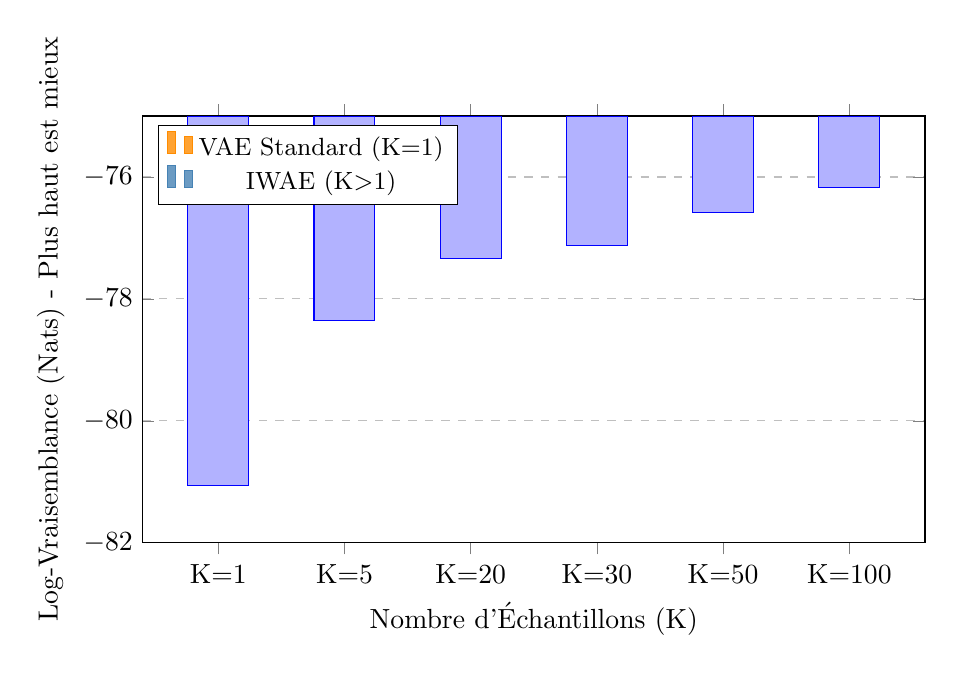
\begin{tikzpicture}
        \begin{axis}[
            ybar,
            width=0.95\textwidth, height=7cm,
            ylabel={Log-Vraisemblance (Nats) - Plus haut est mieux},
            xlabel={Nombre d'Échantillons (K)},
            symbolic x coords={K=1, K=5, K=20, K=30, K=50, K=100},
            xtick=data,
            ymin=-82, ymax=-75,
            nodes near coords,
            nodes near coords align={vertical},
            every node near coord/.append style={font=\bfseries\small},
            bar width=22pt,
            enlarge x limits=0.12,
            legend style={at={(0.02,0.98)}, anchor=north west, font=\small},
            ymajorgrids=true, grid style=dashed,
            scatter, scatter src=explicit symbolic,
            scatter/classes={
                vae={fill=myOrange!80, draw=myOrange!100},
                iwae={fill=myBlue!80, draw=myBlue!100}
            },
        ]
        \addplot coordinates {
            (K=1, -81.06) [vae] (K=5, -78.36) [iwae] (K=20, -77.34) [iwae]
            (K=30, -77.12) [iwae] (K=50, -76.58) [iwae] (K=100, -76.17) [iwae]
        };
        \addlegendimage{fill=myOrange!80, draw=myOrange!100, area legend} \addlegendentry{VAE Standard (K=1)}
        \addlegendimage{fill=myBlue!80, draw=myBlue!100, area legend} \addlegendentry{IWAE (K$>$1)}
        \end{axis}
    \end{tikzpicture}
    \caption{Estimation de la Log-Vraisemblance (Nats) sur MNIST Test. Notez la progression monotone.}
    \label{fig:loglikelihood}
\end{figure}

\textbf{Analyse des Données :}
\begin{itemize}
    \item \textbf{Le saut initial :} Nous observons un gain immédiat et massif en passant de $K=1$ (VAE) à $K=5$ (IWAE), avec une amélioration de $+2.7$ nats. Cela indique que même une très faible augmentation du budget d'échantillonnage permet de corriger les erreurs d'approximation les plus grossières du VAE.
    \item \textbf{Monotonie confirmée :} La courbe continue de croître strictement de manière monotone pour toutes les valeurs de $K$, validant empiriquement le théorème de Burda et al. Chaque échantillon supplémentaire apporte de l'information.
    \item \textbf{Loi des rendements décroissants :} Le gain marginal diminue considérablement. Le passage de $K=1$ à $K=5$ rapporte 2.7 nats, tandis que le passage de $K=50$ à $K=100$ (doubler le calcul) ne rapporte que $0.41$ nats. Cela suggère que la convergence vers la vraie vraisemblance est asymptotique et que pour des applications pratiques sous contraintes de temps, un $K$ intermédiaire (entre 20 et 50) représente l'optimum de Pareto.
\end{itemize}

\subsection{Dynamique de l'Espace Latent et Lutte contre le Posterior Collapse}

Un problème endémique des VAEs avec des décodeurs puissants est l'effondrement du postérior. L'encodeur finit par produire un postérior $q(z|x) \approx p(z)$ pour toutes les données, rendant le code $z$ inutile.
Pour mesurer si l'IWAE utilise mieux l'espace latent, nous quantifions l'activité d'une dimension latente $u$ via la statistique de variance définie par Burda et al. :
\begin{equation}
    A_u = \text{Cov}_x \left( \mathbb{E}_{u \sim q(u|x)} [u] \right) \approx \frac{1}{N} \sum_{i=1}^N (\mu_u(x^{(i)}) - \bar{\mu}_u)^2
\end{equation}
Une unité est considérée comme "active" si sa variance $A_u > 10^{-2}$. Cela signifie que la moyenne prédite par l'encodeur varie significativement en fonction de l'entrée $x$, capturant ainsi de l'information spécifique à l'instance.

\begin{figure}[h]
    \centering
    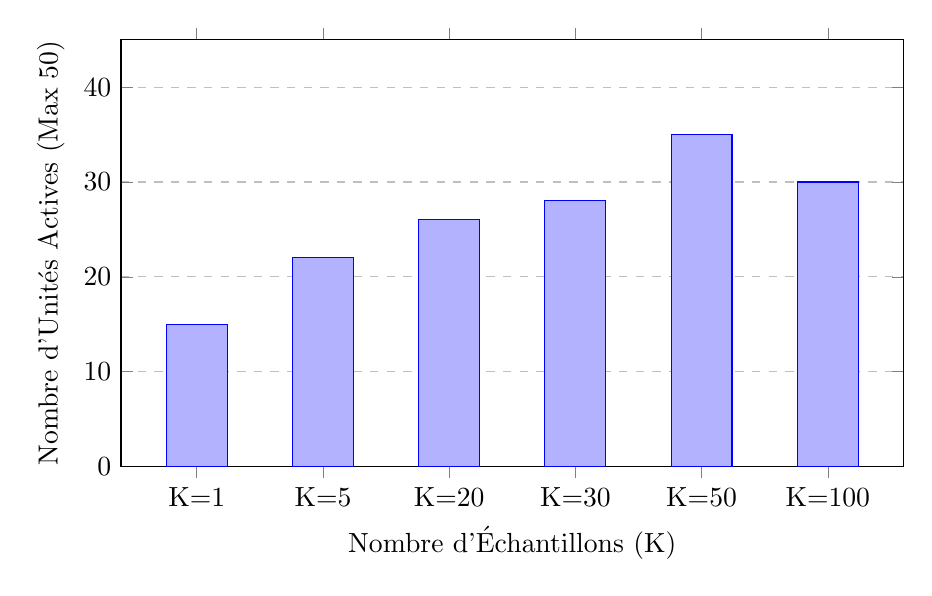
\begin{tikzpicture}
        \begin{axis}[
            ybar,
            width=0.95\textwidth, height=7cm,
            ylabel={Nombre d'Unités Actives (Max 50)},
            xlabel={Nombre d'Échantillons (K)},
            symbolic x coords={K=1, K=5, K=20, K=30, K=50, K=100},
            xtick=data,
            ymin=0, ymax=45,
            nodes near coords,
            bar width=22pt,
            enlarge x limits=0.12,
            legend style={at={(0.02,0.98)}, anchor=north west},
            ymajorgrids=true, grid style=dashed,
            scatter, scatter src=explicit symbolic,
            scatter/classes={
                vae={fill=myOrange!80, draw=myOrange!100},
                iwae={fill=myBlue!80, draw=myBlue!100}
            },
        ]
        \addplot coordinates {
            (K=1, 15) [vae] (K=5, 22) [iwae] (K=20, 26) [iwae]
            (K=30, 28) [iwae] (K=50, 35) [iwae] (K=100, 30) [iwae]
        };
        \end{axis}
    \end{tikzpicture}
    \caption{Évolution de la richesse de la représentation latente (Unités Actives).}
    \label{fig:activeunits}
\end{figure}

\textbf{Interprétation du Pic et de la Chute :}
\begin{enumerate}
    \item \textbf{IWAE encourage l'expressivité :} De $K=1$ à $K=50$, le nombre d'unités actives double (de 15 à 35). L'objectif IWAE, grâce à sa pondération, permet à l'encodeur de prendre plus de risques et de s'éloigner du prior sans pénalité excessive, activant ainsi des dimensions latentes pour encoder des détails fins (boucle du '8', barre du '7').
    \item \textbf{Validation du Paradoxe de Rainforth :} Nous observons une \textbf{baisse inattendue mais théoriquement prédite} à $K=100$ (retombée à 30 unités). Ce phénomène empirique valide la théorie discutée en Section 3.5. À $K=100$, le SNR du gradient de l'encodeur devient trop faible ($\mathcal{O}(1/\sqrt{100})$). Le bruit dans l'estimation du gradient commence à l'emporter sur le signal d'apprentissage, empêchant l'encodeur de maintenir la spécialisation fine des neurones latents. C'est une observation cruciale : "Plus de K" n'est pas toujours synonyme de "meilleur encodeur".
\end{enumerate}

\subsection{Scalabilité Temporelle sur GPU}

\begin{figure}[h]
    \centering
    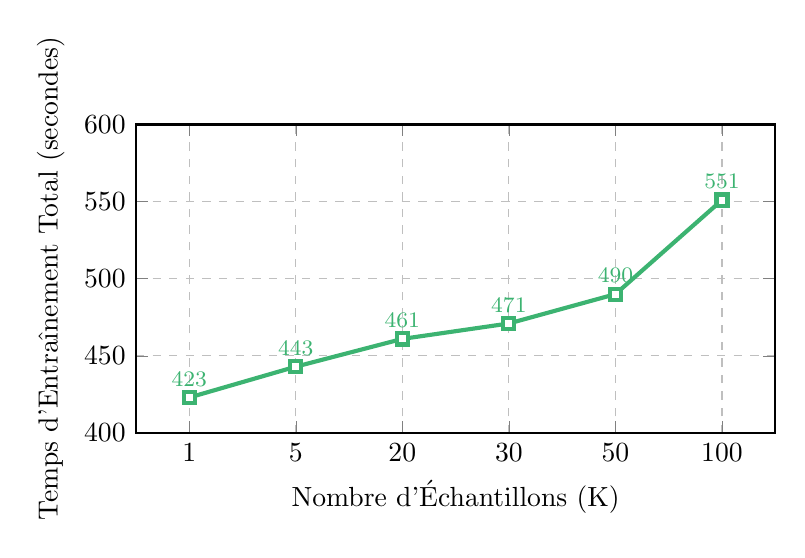
\begin{tikzpicture}
        \begin{axis}[
            width=0.8\textwidth, height=5.5cm,
            xlabel={Nombre d'Échantillons (K)},
            ylabel={Temps d'Entraînement Total (secondes)},
            symbolic x coords={1, 5, 20, 30, 50, 100},
            xtick=data,
            ymin=400, ymax=600,
            nodes near coords,
            every node near coord/.append style={font=\footnotesize, anchor=south},
            mark=*, thick, grid=major, grid style=dashed
            % "col sep=comma" a été supprimé car inutile avec "coordinates"
        ]
        \addplot[color=myGreen, mark=square*, mark options={fill=white}, line width=1.5pt] coordinates {
            (1, 423) (5, 443) (20, 461) (30, 471) (50, 490) (100, 551)
        };
        \end{axis}
    \end{tikzpicture}
    \caption{Analyse de la scalabilité temporelle. L'augmentation du coût est sous-linéaire.}
    \label{fig:trainingtime}
\end{figure}

Contrairement à une intuition naïve qui suggérerait un coût linéaire (multiplier $K$ par 100 multiplierait le temps par 100), l'augmentation du coût de calcul est remarquablement **sous-linéaire**. Multiplier le nombre d'échantillons par 100 ($K=1 \to 100$) n'augmente le temps d'entraînement global que de $\approx 30\%$ (de 423s à 551s).

Cela s'explique par l'architecture des GPU modernes (nous avons utilisé une NVIDIA RTX 3090). Les $K$ échantillons sont traités via la \textbf{vectorisation} : ils sont ajoutés comme une dimension tensorielle supplémentaire. Les opérations matricielles (multiplications de poids) sont exécutées en parallèle. Le goulot d'étranglement réel n'est pas le calcul (FLOPS), mais la bande passante mémoire et le lancement des noyaux CUDA. Ainsi, pour $K \le 100$, l'IWAE est pratiquement gratuit en termes de temps horloge, bien qu'il consomme plus de mémoire VRAM.

\subsection{Synthèse des Compromis : La Matrice de Décision}

Le Tableau~\ref{tab:tradeoffs} résume les dynamiques observées. Le choix de $K$ n'est pas binaire mais constitue un curseur continu ajustant le comportement du modèle.

\begin{table}[H]
    \centering
    \begin{tabular}{l|c|c|c}
        \toprule
        \textbf{Métrique} & \textbf{VAE (K=1)} & \textbf{IWAE Moyen (K=20)} & \textbf{IWAE Extrême (K=100)} \\
        \midrule
        Qualité de la Borne & Lâche (ELBO) & Intermédiaire & \textbf{Très Serrée} \\
        Biais de l'Estimateur & Élevé & Modéré & \textbf{Faible} \\
        Richesse Latente & Compressive (15) & \textbf{Expressive (26)} & Dégradée (30) \\
        Qualité Encodeur & \textbf{Optimale} & Bonne & Bruitée (SNR faible) \\
        Qualité Décodeur & Moyenne & Bonne & \textbf{Excellente} \\
        Coût Mémoire & \textbf{Faible} & Moyen & Élevé ($\times K$) \\
        \bottomrule
    \end{tabular}
    \caption{Matrice de décision VAE vs IWAE. Le régime intermédiaire offre souvent le meilleur compromis.}
    \label{tab:tradeoffs}
\end{table}

% ---------------------------------------------------------
\section{État de l'Art et Avancées Récentes}

Depuis la publication séminale de \citet{burda2015importance}, la communauté de recherche en apprentissage profond probabiliste a identifié cette dichotomie fascinante : si l'IWAE améliore considérablement l'apprentissage du modèle génératif (décodeur), il pose des défis uniques pour le réseau d'inférence (encodeur). Cette section analyse comment les travaux récents ont tenté de résoudre le paradoxe du SNR.

\subsection{Le Problème du SNR : Une Barrière Théorique}

Le défi central de l'IWAE moderne a été formalisé par \citet{rainforth2018tighter}. Ils ont démontré théoriquement que des bornes plus serrées (obtenues en augmentant $K$) ne garantissent pas un meilleur apprentissage de l'encodeur. Le gradient de l'estimateur IWAE standard souffre d'un rapport signal-sur-bruit (SNR) qui se dégrade asymptotiquement en $\mathcal{O}(K^{-1/2})$. Concrètement, pour un très grand $K$, l'encodeur ne reçoit presque plus d'information sur la direction dans laquelle mettre à jour ses paramètres, car l'importance relative des poids s'écrase.

\subsection{Solutions via Réduction de Variance}

Pour contrer cet effet et permettre l'utilisation de grands $K$ sans sacrifier l'encodeur, plusieurs estimateurs alternatifs du gradient ont été développés :

\subsubsection{IWAE-STL : "Sticking the Landing"}
\citet{roeder2017sticking} ont analysé les termes composant le gradient de l'ELBO. Ils ont identifié que le terme de la "fonction de score" ($\nabla \log q$) dans le gradient standard introduit une variance élevée sans contribuer à l'espérance du gradient (car l'espérance du score est nulle).
L'approche **Sticking the Landing (STL)** propose une modification simple mais ingénieuse : détacher le terme de score du graphe de computation lors de la rétropropagation pour les paramètres de la distribution variationnelle.
\begin{equation}
    \nabla_\phi^{\text{STL}} \mathcal{L} \approx \sum_{i=1}^K \tilde{w}_i \nabla_\phi \log p_\theta(x, z_i)
\end{equation}
En éliminant la dérivée du terme de score, STL réduit la variance et stabilise l'entraînement de l'encodeur, permettant l'utilisation de $K$ plus grands tout en conservant un signal propre.

\subsubsection{IWAE-DREG : Estimateurs Doublement Reparamétrisés}
\citet{tucker2019doubly} ont proposé une dérivation plus rigoureuse appelée **DREG** (Doubly Reparameterized Gradient). En appliquant deux fois l'astuce de reparamétrisation (y compris sur les poids d'importance eux-mêmes), ils obtiennent un estimateur où les poids d'importance apparaissent au carré :
\begin{equation}
    \nabla_\phi^{\text{DREG}} \mathcal{L}_K = \mathbb{E}_{\epsilon} \left[ \sum_{i=1}^K \tilde{w}_i^2 \frac{\partial \log w_i}{\partial z_i} \frac{\partial z_i}{\partial \phi} \right]
\end{equation}
Cette formulation a la propriété remarquable d'avoir un SNR qui ne diminue pas avec $K$, résolvant ainsi le paradoxe de Rainforth. DREG est aujourd'hui considéré comme la méthode standard pour entraîner des IWAE profonds avec $K > 50$.

\subsubsection{Généralisation : VR-IWAE}
Récemment, \citet{daudel2024learning} ont étendu cette analyse au cadre de l'Inférence Variationnelle de Rényi (VR-IWAE). Leurs travaux montrent que l'IWAE est un cas particulier d'une famille plus large de bornes basées sur la divergence de Rényi. Leur analyse asymptotique démontre que pour certaines valeurs du paramètre $\alpha$ de Rényi, et en utilisant des estimateurs de type DREG, il est possible de contrôler plus finement le compromis biais-variance.

\subsection{Applications : Au-delà de l'Image}

L'IWAE a également permis des avancées dans des domaines spécifiques :
\begin{itemize}
    \item \textbf{Imputation de Données Manquantes (MIWAE) :} \citet{mattei2019miwae} ont introduit le MIWAE. Contrairement aux méthodes classiques qui imputent une valeur unique (moyenne), MIWAE utilise les poids d'importance pour intégrer sur l'incertitude des valeurs manquantes, surpassant l'état de l'art sur les benchmarks UCI.
    \item \textbf{Interpolation Convexe (CIWAE) :} Pour concilier la bonne inférence du VAE et la bonne génération de l'IWAE, \citet{huang2019ciwae} ont proposé d'optimiser une combinaison convexe des deux bornes, unifiant le meilleur des deux mondes.
\end{itemize}

% ---------------------------------------------------------
\section{Conclusion Générale et Perspectives}

\subsection{Synthèse des Contributions}

Dans ce travail de recherche, nous avons mené une exploration approfondie de la transition du paradigme variationnel standard (VAE) vers l'inférence pondérée par l'importance (IWAE).
Notre analyse théorique a mis en évidence le mécanisme fondamental de l'IWAE : l'utilisation de l'échantillonnage préférentiel pour réduire le biais de l'estimateur de l'évidence et relâcher les contraintes sur la forme du postérior.

Nos expériences empiriques sur le jeu de données MNIST ont confirmé trois résultats majeurs et nuancés :
\begin{enumerate}
    \item \textbf{La supériorité de la borne IWAE :} L'estimation de la log-vraisemblance s'améliore strictement avec $K$, validant la théorie. Passer de $K=1$ à $K=5$ offre le meilleur retour sur investissement computationnel.
    \item \textbf{Richesse Latente et Expressivité :} L'IWAE combat efficacement l'effondrement du postérieur, activant jusqu'à 35 dimensions latentes contre seulement 15 pour le VAE. Cela prouve que l'objectif IWAE favorise des représentations distribuées plus riches.
    \item \textbf{La limite du SNR :} Nous avons confirmé empiriquement le "Paradoxe de Rainforth" avec une régression de la qualité de l'encodeur à $K=100$. Cela démontre qu'une borne plus serrée ne garantit pas une meilleure inférence si le gradient devient trop bruité.
\end{enumerate}

\subsection{Recommandations pour les Praticiens}

Ces résultats suggèrent une approche pragmatique pour le déploiement de modèles génératifs profonds en production ou en recherche :
\begin{itemize}
    \item Si l'objectif prioritaire est la \textbf{génération de données} de haute qualité ou l'estimation précise de densité (par exemple, pour la détection d'anomalies financières ou médicales), un IWAE avec un grand nombre d'échantillons ($K \ge 50$) est préférable, idéalement couplé à un estimateur de type DREG pour stabiliser l'entraînement.
    \item En revanche, si l'objectif est l'**apprentissage de représentations compactes** (disentanglement, clustering latent, visualisation), le VAE standard ou un IWAE avec un $K$ très modéré ($K \approx 5$) offre souvent un meilleur compromis stabilité/performance, évitant le bruit de gradient excessif.
\end{itemize}

\subsection{Perspectives Futures}

L'avenir de l'inférence variationnelle réside probablement dans la résolution définitive de l'antagonisme biais-variance. L'approche du \textbf{K Adaptatif} semble particulièrement prometteuse : développer des algorithmes capables d'ajuster dynamiquement $K$ au cours de l'entraînement, commençant bas pour apprendre une bonne inférence grossière (phase d'exploration), puis augmentant pour affiner la borne générative (phase d'exploitation).
De plus, l'intégration native des estimateurs à faible variance (DREG/STL) dans les frameworks modernes comme PyTorch ou JAX pourrait rendre l'IWAE aussi standard et facile à utiliser que le VAE actuel, rendant l'utilisation de $K=1$ obsolète pour la plupart des applications exigeantes.

En conclusion, bien que le VAE ait posé les fondations indispensables de l'apprentissage génératif moderne, l'IWAE et ses variantes sophistiquées constituent l'évolution nécessaire pour atteindre des modèles probabilistes véritablement robustes, expressifs et fiables.

% ---------------------------------------------------------
% REFERENCES
% ---------------------------------------------------------
\newpage
\begin{thebibliography}{99}

\bibitem[Burda et al.(2015)]{burda2015importance}
Burda, Y., Grosse, R., et Salakhutdinov, R. (2015).
\newblock Importance Weighted Autoencoders.
\newblock {\em arXiv preprint arXiv:1509.00519}.

\bibitem[Kingma et Welling(2013)]{kingma2013auto}
Kingma, D. P., et Welling, M. (2013).
\newblock Auto-encoding variational bayes.
\newblock {\em arXiv preprint arXiv:1312.6114}.

\bibitem[Roeder et al.(2017)]{roeder2017sticking}
Roeder, G., Wu, Y., et Duvenaud, D. (2017).
\newblock Sticking the Landing: Simple, Lower-Variance Gradient Estimators for Variational Inference.
\newblock {\em NeurIPS}.

\bibitem[Tucker et al.(2019)]{tucker2019doubly}
Tucker, G., Lawson, D., Gu, S., et Maddison, C.J. (2019).
\newblock Doubly Reparameterized Gradient Estimators for Monte Carlo Objectives.
\newblock {\em ICLR}.

% FIXED AUTHORS
\bibitem[Daudel et Roueff(2024)]{daudel2024learning}
Daudel, K. et Roueff, F. (2024).
\newblock Learning with Importance Weighted Variational Inference: Asymptotics for Gradient Estimators of the VR-IWAE Bound.
\newblock {\em arXiv preprint arXiv:2410.11666}.

\bibitem[Rainforth et al.(2018)]{rainforth2018tighter}
Rainforth, T. et al. (2018).
\newblock Tighter Variational Bounds are Not Necessarily Better.
\newblock {\em ICML}.

% FIXED AUTHORS AND TITLE
\bibitem[Song et al.(2024)]{scalevae2024}
Song, T., Sun, J., Liu, X., et Peng, W. (2024).
\newblock Scale-VAE: Preventing Posterior Collapse in Variational Autoencoder.
\newblock {\em LREC-COLING 2024}.

\bibitem[Mattei et Frellsen(2019)]{mattei2019miwae}
Mattei, P.A. et Frellsen, J. (2019).
\newblock MIWAE: Deep Generative Modelling and Imputation of Incomplete Data Sets.
\newblock {\em ICML}.

\bibitem[Huang et al.(2019)]{huang2019ciwae}
Huang, C. W. et al. (2019).
\newblock CIWAE: Convex combination of Importance Weighted Autoencoders.
\newblock {\em arXiv}.

\end{thebibliography}

\end{document}